\documentclass{standalone}
\usepackage{tikz}
\usetikzlibrary{patterns, positioning}


\begin{document}
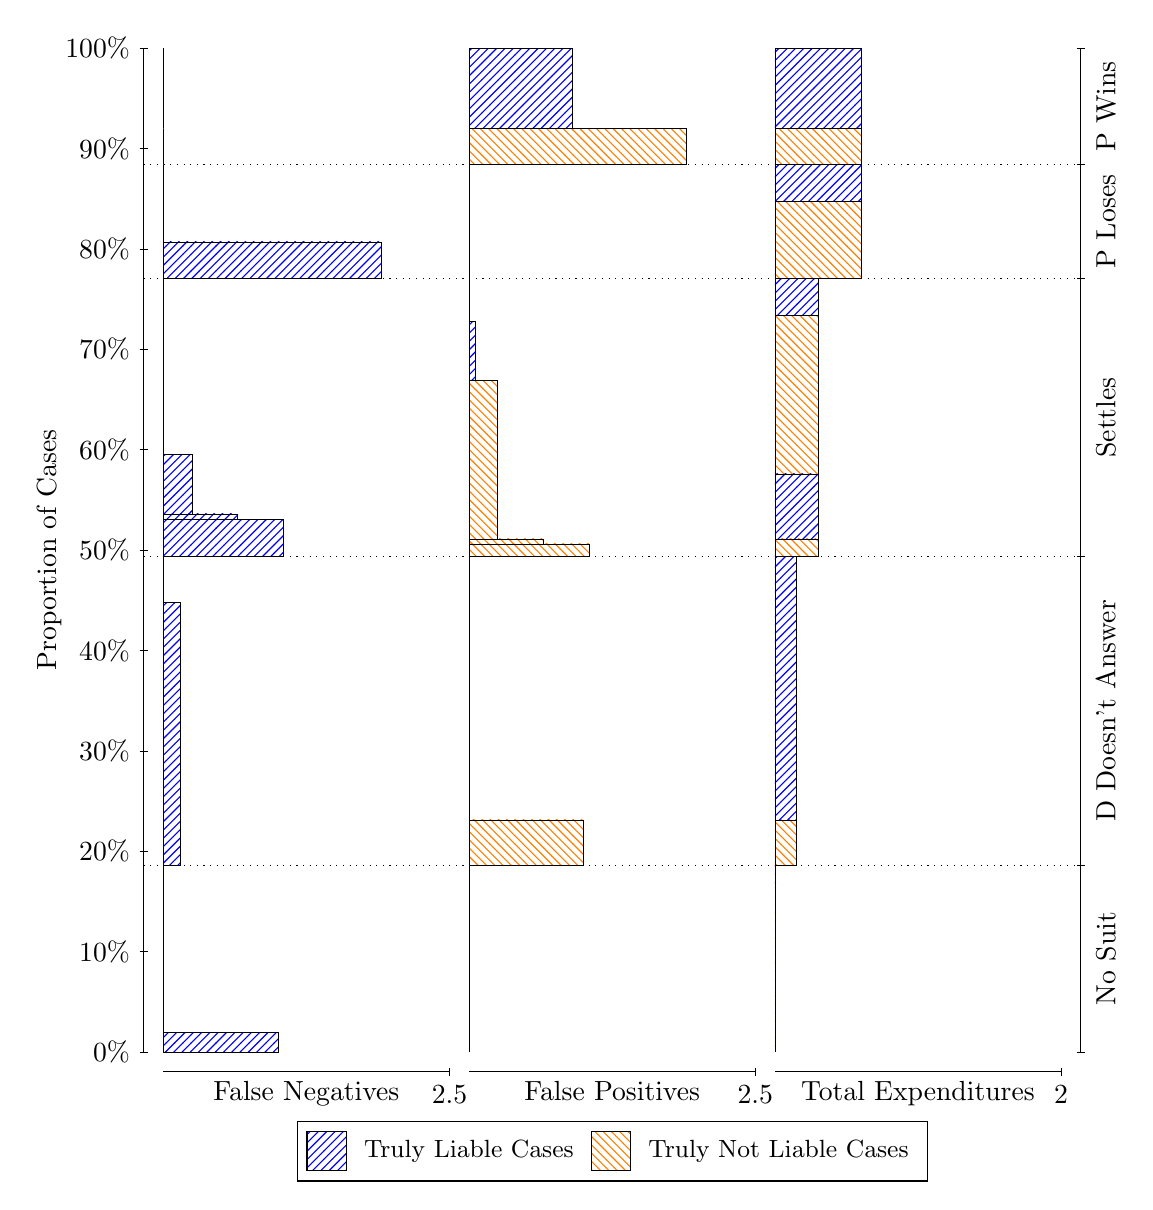
\begin{tikzpicture}
\draw[black, very thin] (1.5,1.75) -- (1.5,14.5);
\node[rotate=90, text=black, anchor=center] at (0.3, 8.125) {Proportion of Cases};
\draw[black, very thin] (1.45,1.75) -- (1.55,1.75);
\node[text=black, anchor=east] at (1.45, 1.75) {0\%};
\draw[black, very thin] (1.45,3.025) -- (1.55,3.025);
\node[text=black, anchor=east] at (1.45, 3.025) {10\%};
\draw[black, very thin] (1.45,4.3) -- (1.55,4.3);
\node[text=black, anchor=east] at (1.45, 4.3) {20\%};
\draw[black, very thin] (1.45,5.575) -- (1.55,5.575);
\node[text=black, anchor=east] at (1.45, 5.575) {30\%};
\draw[black, very thin] (1.45,6.85) -- (1.55,6.85);
\node[text=black, anchor=east] at (1.45, 6.85) {40\%};
\draw[black, very thin] (1.45,8.125) -- (1.55,8.125);
\node[text=black, anchor=east] at (1.45, 8.125) {50\%};
\draw[black, very thin] (1.45,9.4) -- (1.55,9.4);
\node[text=black, anchor=east] at (1.45, 9.4) {60\%};
\draw[black, very thin] (1.45,10.675) -- (1.55,10.675);
\node[text=black, anchor=east] at (1.45, 10.675) {70\%};
\draw[black, very thin] (1.45,11.95) -- (1.55,11.95);
\node[text=black, anchor=east] at (1.45, 11.95) {80\%};
\draw[black, very thin] (1.45,13.225) -- (1.55,13.225);
\node[text=black, anchor=east] at (1.45, 13.225) {90\%};
\draw[black, very thin] (1.45,14.5) -- (1.55,14.5);
\node[text=black, anchor=east] at (1.45, 14.5) {100\%};

\draw[black, very thin] (13.4,1.75) -- (13.4,14.5);
\draw[black, very thin] (13.35,1.75) -- (13.45,1.75);
\node[anchor=west] at (13.35, 1.75) {};
\draw[black, very thin] (13.35,4.1224) -- (13.45,4.1224);
\node[anchor=west] at (13.35, 4.1224) {};
\draw[black, very thin] (13.35,8.0397) -- (13.45,8.0397);
\node[anchor=west] at (13.35, 8.0397) {};
\draw[black, very thin] (13.35,11.577) -- (13.45,11.577);
\node[anchor=west] at (13.35, 11.577) {};
\draw[black, very thin] (13.35,13.018) -- (13.45,13.018);
\node[anchor=west] at (13.35, 13.018) {};
\draw[black, very thin] (13.35,14.5) -- (13.45,14.5);
\node[anchor=west] at (13.35, 14.5) {};

\draw[black, very thin, pattern color=blue, pattern=north east lines] (1.75,1.75) rectangle (3.2033,1.9996);
\draw[black, very thin, pattern color=orange, pattern=north west lines] (1.75,1.9996) rectangle (1.75,4.1224);
\draw[black, very thin, pattern color=blue, pattern=north east lines] (1.75,4.1224) rectangle (1.968,7.4637);
\draw[black, very thin, pattern color=orange, pattern=north west lines] (1.75,7.4637) rectangle (1.75,8.0397);
\draw[black, very thin, pattern color=blue, pattern=north east lines] (1.75,8.0397) rectangle (3.276,8.5153);
\draw[black, very thin, pattern color=blue, pattern=north east lines] (1.75,8.5153) rectangle (2.6947,8.585);
\draw[black, very thin, pattern color=blue, pattern=north east lines] (1.75,8.585) rectangle (2.1133,9.342);
\draw[black, very thin, pattern color=orange, pattern=north west lines] (1.75,9.342) rectangle (1.75,11.577);
\draw[black, very thin, pattern color=blue, pattern=north east lines] (1.75,11.577) rectangle (4.5113,12.039);
\draw[black, very thin, pattern color=orange, pattern=north west lines] (1.75,12.039) rectangle (1.75,13.018);
\draw[black, very thin, pattern color=orange, pattern=north west lines] (1.75,13.018) rectangle (1.75,13.481);
\draw[black, very thin, pattern color=blue, pattern=north east lines] (1.75,13.481) rectangle (1.75,14.5);
\draw[black, very thin, pattern color=orange, pattern=north west lines] (5.6333,1.75) rectangle (5.6333,3.8728);
\draw[black, very thin, pattern color=blue, pattern=north east lines] (5.6333,3.8728) rectangle (5.6333,4.1224);
\draw[black, very thin, pattern color=orange, pattern=north west lines] (5.6333,4.1224) rectangle (7.0867,4.6984);
\draw[black, very thin, pattern color=blue, pattern=north east lines] (5.6333,4.6984) rectangle (5.6333,8.0397);
\draw[black, very thin, pattern color=orange, pattern=north west lines] (5.6333,8.0397) rectangle (7.1593,8.2035);
\draw[black, very thin, pattern color=orange, pattern=north west lines] (5.6333,8.2035) rectangle (6.578,8.2653);
\draw[black, very thin, pattern color=orange, pattern=north west lines] (5.6333,8.2653) rectangle (5.9967,10.275);
\draw[black, very thin, pattern color=blue, pattern=north east lines] (5.6333,10.275) rectangle (5.706,11.032);
\draw[black, very thin, pattern color=blue, pattern=north east lines] (5.6333,11.032) rectangle (5.6333,11.577);
\draw[black, very thin, pattern color=orange, pattern=north west lines] (5.6333,11.577) rectangle (5.6333,12.556);
\draw[black, very thin, pattern color=blue, pattern=north east lines] (5.6333,12.556) rectangle (5.6333,13.018);
\draw[black, very thin, pattern color=orange, pattern=north west lines] (5.6333,13.018) rectangle (8.3947,13.481);
\draw[black, very thin, pattern color=blue, pattern=north east lines] (5.6333,13.481) rectangle (6.9413,14.5);
\draw[black, very thin, pattern color=orange, pattern=north west lines] (9.5167,1.75) rectangle (9.5167,3.8728);
\draw[black, very thin, pattern color=blue, pattern=north east lines] (9.5167,3.8728) rectangle (9.5167,4.1224);
\draw[black, very thin, pattern color=orange, pattern=north west lines] (9.5167,4.1224) rectangle (9.7892,4.6984);
\draw[black, very thin, pattern color=blue, pattern=north east lines] (9.5167,4.6984) rectangle (9.7892,8.0397);
\draw[black, very thin, pattern color=orange, pattern=north west lines] (9.5167,8.0397) rectangle (10.062,8.2653);
\draw[black, very thin, pattern color=blue, pattern=north east lines] (9.5167,8.2653) rectangle (10.062,9.0921);
\draw[black, very thin, pattern color=orange, pattern=north west lines] (9.5167,9.0921) rectangle (10.062,11.101);
\draw[black, very thin, pattern color=blue, pattern=north east lines] (9.5167,11.101) rectangle (10.062,11.577);
\draw[black, very thin, pattern color=orange, pattern=north west lines] (9.5167,11.577) rectangle (10.607,12.556);
\draw[black, very thin, pattern color=blue, pattern=north east lines] (9.5167,12.556) rectangle (10.607,13.018);
\draw[black, very thin, pattern color=orange, pattern=north west lines] (9.5167,13.018) rectangle (10.607,13.481);
\draw[black, very thin, pattern color=blue, pattern=north east lines] (9.5167,13.481) rectangle (10.607,14.5);
\draw[black, dotted] (1.5,4.1224) -- (13.4,4.1224);
\draw[black, dotted] (1.5,8.0397) -- (13.4,8.0397);
\draw[black, dotted] (1.5,11.577) -- (13.4,11.577);
\draw[black, dotted] (1.5,13.018) -- (13.4,13.018);
\draw[black, very thin] (1.75,1.5) -- (5.3833,1.5);
\node[text=black, anchor=north] at (3.5667, 1.5) {False Negatives};
\draw[black, very thin] (5.3833,1.45) -- (5.3833,1.55);
\node[text=black, anchor=north] at (5.3833, 1.45) {2.5};

\draw[black, very thin] (5.6333,1.5) -- (9.2667,1.5);
\node[text=black, anchor=north] at (7.45, 1.5) {False Positives};
\draw[black, very thin] (9.2667,1.45) -- (9.2667,1.55);
\node[text=black, anchor=north] at (9.2667, 1.45) {2.5};

\draw[black, very thin] (9.5167,1.5) -- (13.15,1.5);
\node[text=black, anchor=north] at (11.333, 1.5) {Total Expenditures};
\draw[black, very thin] (13.15,1.45) -- (13.15,1.55);
\node[text=black, anchor=north] at (13.15, 1.45) {2};

\node[text=black, centered, rotate=90] at (13.72, 2.9362) {No Suit};
\node[text=black, centered, rotate=90] at (13.72, 6.081) {D Doesn't Answer};
\node[text=black, centered, rotate=90] at (13.72, 9.8083) {Settles};
\node[text=black, centered, rotate=90] at (13.72, 12.298) {P Loses};
\node[text=black, centered, rotate=90] at (13.72, 13.759) {P Wins};

\draw (7.449999999999999,1.5) node[draw=none] (baseCoordinate) {};
\begin{scope}[align=center]
        \matrix[scale=0.5, draw=black, below=0.5cm of baseCoordinate, nodes={draw}, column sep=0.1cm]{
            \node[rectangle, draw, minimum width=0.5cm, minimum height=0.5cm, pattern color=blue, pattern=north east lines] {}; &
            \node[draw=none, font=\small, text=black] (B) {Truly Liable Cases}; &
            \node[rectangle, draw, minimum width=0.5cm, minimum height=0.5cm, pattern color=orange, pattern=north west lines] {}; &
            \node[draw=none, font=\small, text=black] (B) {Truly Not Liable Cases}; \\
            };
\end{scope}

\end{tikzpicture}
\end{document}